\subsection{Axiale Moden}
\subsubsection{Messung des Modenabstands}
Um die axialen Moden zu messen, wurde der Laserstrahl in das Fabry-Perot Interferometer umgelenkt.
Dieser befindet sich dabei im Mulit-Mode Betrieb.\\
Der Modenabstand zweier axialer Lasermoden $\left(\Delta\nu\right)_M$ lässt sich durch die Resonatorlänge $L$ (Abstand zwischen den Spiegeln im Laser) berechnen.
Die entsprechende Formel wurde bereits in der Theorie diskutiert:
\begin{equation}
    \left(\Delta\nu\right)_{theo.}=\frac{c}{2Ln}
\end{equation}
Somit folgt (mit einer Näherung des Brechungsindexes $n \approx 1$): %%%%%%%Linken%%%%%%
\begin{equation}
    \left(\Delta\nu\right)_{theo.} = \left(275\pm10\right)\,\text{MHz}
\end{equation}
Um den Modenabstand bestimmen zu können muss erst eine Umrechnungsformel hergeleitet werden, damit man die gemessenen Zeitabstände in Frequenzen umrechnen kann.
Zuerst wird der Abstand zweier 'Moden-Blöcke' gemessen:
\begin{figure}[h]
    \centering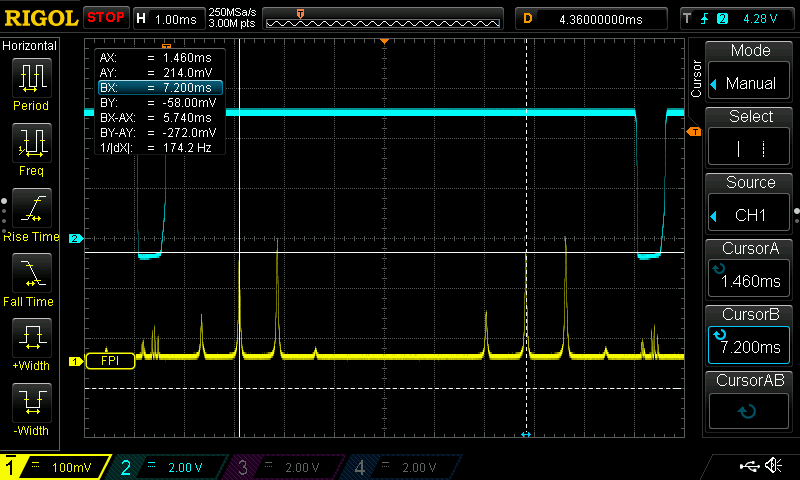
\includegraphics[width=0.7\textwidth]{Auswertung-Dominik/DS1Z_QuickPrint1.png}
    \caption{Messung des Abstandes zweier Moden-Blöcke}
\end{figure}\\
Auf den Oszilloskop sieht man zwei, vom FPI gemessene, Modenblöcke.
Auf der y-Achse ist die Intensität und auf der x-Achse die zeitliche Einteilung der Messung aufgetragen.
Um möglichst genau messen zu können, wurde vor jeder Messung kurz die Luft angehalten und stillgestanden (Damit die Bewegungen die Resonatorlänge nicht verändern) und ein Standbild des Oszilloskopbildschirms gemacht, welcher danach vermessen wurde.
Der Abstand zweier Modenblöcke wurde mit $\Delta t_{FPI}=5,74\,\text{ms}$, durch die beiden Cursor gemessen.
Als Fehler wird immer ein Ablesefehler, die kleinste mögliche ablesbare Einheit, angenommen.
Mit den aus der Versuchsanleitung bekannten Wert für die FRS (free spectral range) des Fabry-Perot-Interferometer ($FSR=2\,\text{GHz}$) folgt für die Umrechnungsformel:
\begin{equation}
    \nu=\frac{x}{5,74\cdot10^{-3}\,\text{s}}\cdot\left(2\,\text{GHz}\right)
\end{equation}
Wobei $x$ für den gemessen Zeitwert steht.\\

Nun wird der Abstand zweier Moden gemessen:
\begin{figure}[h]
    \centering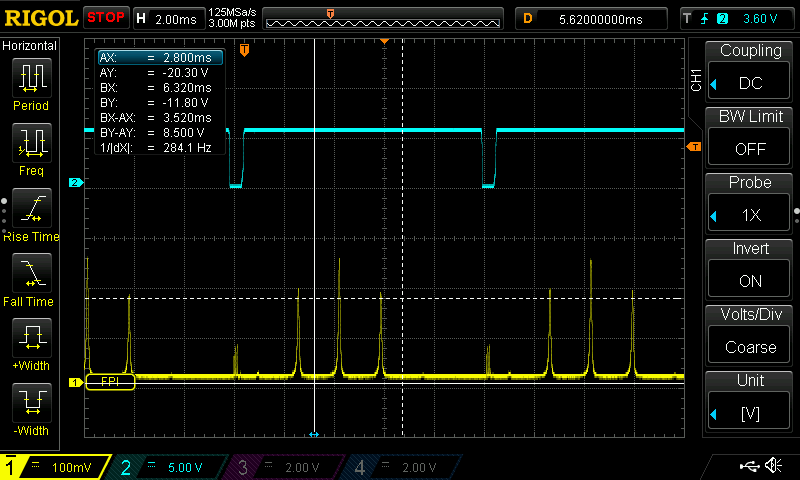
\includegraphics[width=0.7\textwidth]{Auswertung-Dominik/DS1Z_QuickPrint2.png}
    \caption{Messung des Abstandes zweier Moden}
\end{figure}\\
Hier wurde mit dem Oszilloskop ein Abstand, zwischen zwei benachbarten Moden, von $776\,\mu s$ gemessen.
Dabei wurde darauf geachtet, dass die Cursor des Oszilloskops mittig in den Peaks stehen.
Somit folgt als realer Modenabstand:
\begin{equation}
    \left(\Delta\nu\right)_M=\left(270,38\pm0,59\right)\,\text{MHz}
\end{equation}
Als Ablesefehler wurde wieder die kleinste veränderliche Einheit gewählt.
Der Fehler wurde über Fehlerfortpflanzung bestimmt, siehe Anhang.
Der Wert für den Modenabstand liegt somit im Fehlerbereich des theoretisch erwarteten Wertes.\newpage

Die Breite einer Mode wird analog bestimmt:
\begin{figure}[h]
    \centering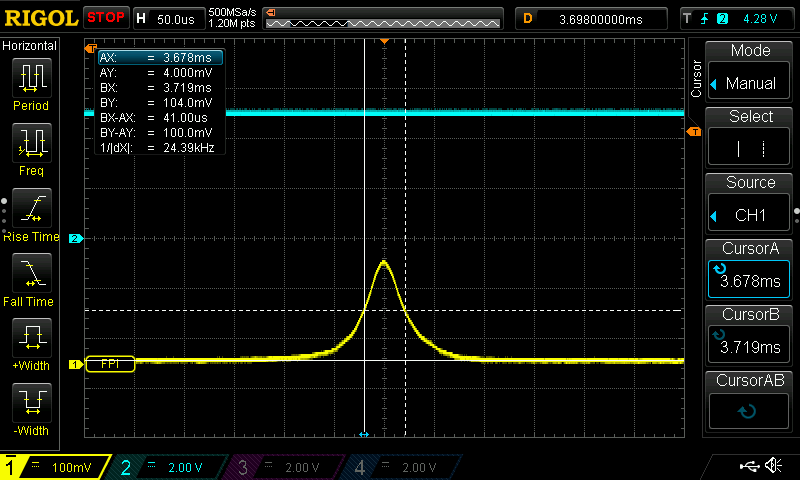
\includegraphics[width=0.7\textwidth]{Auswertung-Dominik/DS1Z_QuickPrint4.png}
    \caption{Messung Breite einer Mode im multi-mode Betrieb}
\end{figure}\\
Die Halbwertsbreite wurde mit $41\,\mu s$ gemessen. Hierbei musste man beachten, dass man die Cursor so platziert das diese in den Schnittpunkten zwischen der Mode und der halben Maximumsintensität (waagrechte gestrichelte Linie) liegen.\\
Somit folgt für die Breite der Mode:
\begin{equation}
    \left(\Delta\nu\right)_m=\left(14,0\pm0,3\right)\,\text{MHz}
\end{equation}
Die Ablesegenauigkeit ist wiederum die kleinste veränderliche Einheit und der Fehler wurde analog wie zuvor bestimmt.\newpage
Der Laser wurde in den Singe-mode Betrieb geschalten.\\
Für die Breite einer Mode folgt nun:
\begin{figure}[h]
    \centering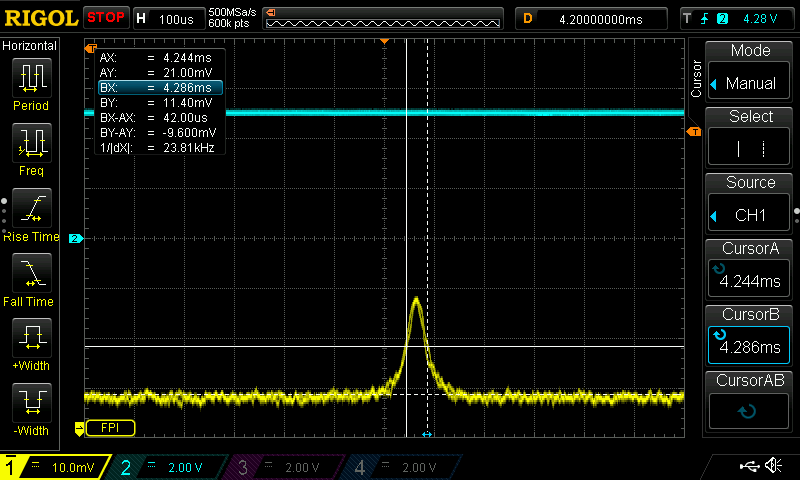
\includegraphics[width=0.7\textwidth]{Auswertung-Dominik/DS1Z_QuickPrint7.png}
    \caption{Messung Breite einer Mode im single-mode Betrieb}    
\end{figure}\\
Die Halbwertsbreite wurde mit $42\,\mu s$ gemessen.
Dabei wurde wie im Multimode-Betrieb darauf geachtet, dass man auf der Höhe der halben Maximumsintensität die Breite der Mode misst.
Im single-mode Betrieb war es deutlich schwerer ein Standbild zu finden, wo die Mode an sich nicht zu unscharf war.
Bei unserer Aufnahme kann man noch leicht sehen, dass diese noch etwas am zittern war.\\
Für die Breite dieser folgt:
\begin{equation}
    \left(\Delta\nu\right)_m=\left(14,6\pm0,3\right)\,\text{MHz}
\end{equation}
Ablesefehler und Fehlerfortpflanzung sind analog zu den zuvor berechneten Werten.\newpage
\subsubsection{Breite des Verstärkungsprofils}
Die Breite des Verstärkungsprofils (wieder im mulit-mode Betrieb) lässt sich am Oszilloskop sichtbar machen, indem man den Versuchstisch ruckartig bewegt, da die Lasermoden anfällig gegenüber Erschütterungen sind.
Hierbei wird eine 'Langzeitaufnahme' am Oszilloskop aufgenommen und das Verstärkungsprofils zeichnet sich ab:
\begin{figure}[h]
    \centering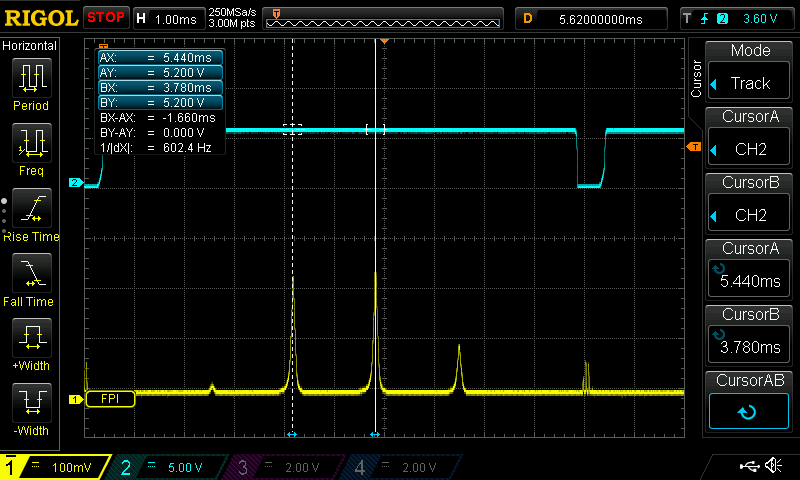
\includegraphics[width=0.7\textwidth]{Auswertung-Dominik/DS1Z_QuickPrint6.png}
    \caption{Messung des Verstärkungsprofils}
\end{figure}\\
Hier wurde die zu erwartete Gaußkurve zu extrapoliert und dann die Halbwertsbreite ($1,75\,\text{ms}$) abgelesen.
Somit folgt für die Verstärkung:
\begin{equation}
    \left(\Delta\nu\right)_\text{Verst}=\left(610\pm4\right)\,\text{MHz}
\end{equation}
Der gemessene Wert ist kleiner als der freie Spektralbereich des FPI, dies war auch zu erwarten. Ansonsten würden sich die axialen Moden überlagern und wären so nicht mehr trennbar.
\subsubsection{Auflösevermögen}
Das Auflösevermögen $A$ lässt sich mit dem Verhältnis der Frequenz des Lasers zu der Linienbreite bestimmen:
\begin{equation}
    A=\frac{\nu}{\Delta\nu_m}=\frac{c}{\lambda\cdot\Delta\nu_m}=\left(33,8\pm0,7\right)\cdot10^6
\end{equation}
Die Finesse $F$ des FPI ist das Verhältnis vom freien Spektralbereich zur Linienbreite:
\begin{equation}
    F=\frac{FSR}{\Delta\nu_m}=\left(142,9\pm3,1\right)
\end{equation}\newpage
\subsubsection{Messungen mit einer schnellen Photodiode}
%Der Laser läuft im singe-mode Betrieb.
%Hierbei lässt sich der Modenabstand messen, indem die Schwebungsfrequenz, der sich überlagernden Moden, mit einer schnellen Photodiode und einem Spektrumanalysator gemessen wird.
%Die durch den Laser verursachte Linie lässt sich im Spektrum finden, indem der Laserstrahl abwechselnd blockiert und wieder freigegeben wird, zusätzlich wird noch auf einen verschwindenden Peak im Spektrum geachtet.\\
Bei der Messung mit einer schnellen Photodiode wird die Schwebungsfrequenz zweier Axialer Moden (im mulit-mode Betrieb) mithilfe des Spektrumanalysators gemessen.
Die durch den Laser verursachte Linie lässt sich im Spektrum finden, indem der Laserstrahl abwechselnd blockiert und wieder freigegeben wird, zusätzlich wird noch auf einen verschwindenden Peak im Spektrum geachtet.\\
Ohne Plättchen misst man folgendes Spektrum:
\begin{figure}[h]
    \centering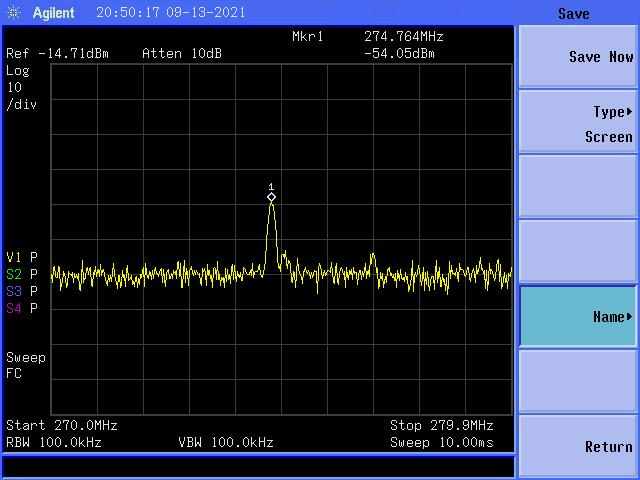
\includegraphics[width=0.7\textwidth]{Auswertung-Dominik/BB.JPG}
    \caption{Spektrum ohne Glasplättchen, Marker auf Schwebungsfrequenz}
\end{figure}\\
Hier wird eine Schwebungsfrequenz von $\Delta\nu_{S1}=\left(274,764\pm0,001\right)\,\text{MHz}$ gemessen.
Der Ablesefehler ist wiederum die kleinste veränderliche Einheit. %Dies ist vergleichbar mit dem Abstand der Moden.
Das gemessene Ergebnis liegt im Fehlerbereich des theoretisch zu erwarteten.\\

Der Modenabstand hängt von der Resonatorlänge ab.
Nun wird ein Glasplättchen in den Resonator eingebracht und somit die Resonatorlänge verändert.
Durch diese Veränderung verändert sich auch die Schwebungsfrequenz der Moden.
Hiermit kann man die Dicke des Glasplättchen wie folgt berechnen:
\begin{equation}
    d=L_2-L_1=\frac{c}{2n}\left(\frac{1}{\Delta\nu_{S2}}-\frac{1}{\Delta\nu_{S1}}\right)
\end{equation}\newpage
Wenn nun das Glasplättchen eingebracht ist, ändert sich die Schwebungsfrequenz wie folgt:
\begin{figure}[h]
    \centering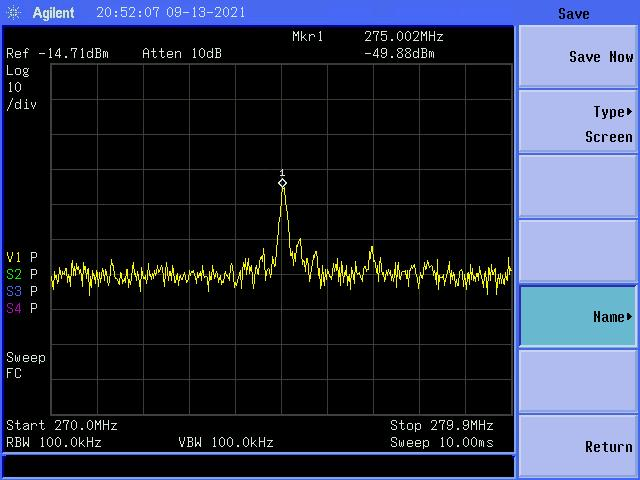
\includegraphics[width=0.7\textwidth]{Auswertung-Dominik/ABC.JPG}
    \caption{Spektrum mit Glasplättchen, Marker auf Schwebungsfrequenz}
\end{figure}\\
Mit dem 1983 definierten Wert für die Lichtgeschwindigkeit ($c=299792458\,\text{m/s}$), dem gemessenen Wert $\Delta\nu_{S2}=275,002\,\text{MHz}$ und der Vernachlässigung des Brechungsindexes folgt:
\begin{equation}
    d=\left(472\pm22\right)\,\mu m
\end{equation}
Die Messung ist aufgrund des verwendeten Spektrumanalysators sehr ungenau.
Das Ergebnis liegt zwar in der Größenordnung des realen Wertes, ist aber trotzdem um das Zweifache größer.
Um ein genaueres Ergebnis zu bekommen, müsste man versuchen die Störfrequenzen zu beseitigen, damit man die eigentliche Frequenz auf dem Spektrumanalysator besser und genauer bestimmen kann.\\

Hätte man nun eine Einstell- und Ablesegenauigkeit von $100\,\text{Hz}$, so folgt für die Genauigkeit der Dicke nach der Fehlerfortpflanzung:
\begin{align}
    s_d&=\frac{c}{2n}\sqrt{\left(\frac{100\,\text{Hz}}{\Delta\nu_{S2}^2}\right)^2+\left(\frac{100\,\text{Hz}}{\Delta\nu_{S1}^2}\right)^2+\left(\frac{s_n}{n}\left(\frac{1}{\Delta\nu_{S2}}-\frac{1}{\Delta\nu_{S1}}\right)\right)^2}\\
    s_d&=13,1\,\mu m
\end{align}
\newpage